\chapter{前言}
\section{应用背景:协同编辑应用}
	\par 协同编辑系统,如 Google Docs, Apache Wave, wikis 等可以允许不同地点的用户同时编辑同一份文档。为了获得较快的响应和较高的实用性,系统会在不同的地点或设备进行文档的复制。一个用户可以在某个副本上进行文档的编辑,并将做出的修改异步地传递给其他副本。不必要等待服务器处理完再响应用户操作,本地操作可以立即执行。同时系统必须保证编辑的一致性,即在所有用户完成文档的编辑后,所有的副本内容一致。

\section{技术背景:Replicated List 规约及其基于OT的 Replicated List 算法}

\subsection{规约}
List 支持的常见简单操作 (insert, del, read)

规约: convergence (strong eventual consistency)
Def2 and Def3 of ``SSS''
Definition. A groupware session is quiescent iff all generated
operations have been executed at all sites, that is, there
are no requests in transit or waiting to be executed by a
site process.\cite{ellis1989concurrency}

Definition. The Convergence Property states that site objects
are identical at all sites at quiescence.\cite{ellis1989concurrency}

\subsection{OT}
Operational Transformation(OT)是一种为了支持协作功能,在协作软件系统中所采用的技术。OT最早在1989年被提出,是为了在纯文本文档的协同编辑中实现一致性和并发控制所发明的,经过二十余年的研究,OT的能力已经得到了拓展,在2009年OT做为一种核心技术被Apache Wave和Google Docs所采用来实现其合作特点。
OT的基本思想是根据先前执行的并发操作的影响,对正在编辑的操作的参数进行转换或调整,是转换后的操作能够达到正确地操作,并且保持文档的一致性。
在这里举一个简单的例子说明OT的思想:
\begin{figure}[H]
\centering
\includegraphics{figures/exm1.bmp}
\caption{不使用OT}
\end{figure}
在某个状态S时,list内容为”ABCDE",此时client端执行了一个删除第4个字符的操作,server端执行了一个删除第2个字符的操作,如图所示,client端list的内容变为“ABCE”,server端list的内容变为“ACDE”。如果不进行转换,直接将操作相互传递,则client端接受到的操作是删除第2个字符,server端接受到的操作是删除第4个字符,完成操作后client端list的内容为“ACE”,server端list的内容为“ACD”,此时list的内容不同,不满足一致性。其原因在于client端的删除第4个字符的操作应该是删除D,但是传递到server端时,由于没有进行操作的转换,此时删除第4个字符即删除E,造成了删除内容的不一致。
\begin{figure}[H]
\centering
\includegraphics{figures/exm2.bmp}
\caption{使用OT}
\end{figure}
使用OT技术将$Del\ 4$转换为$Del\ 3$,$Del\ 2$转换为$Del\ 2$,这样操作的传递完成后,文档的内容仍然是一致的。

\subsection{OT-based 协议}
client-server 结构

一个OT系统包含2个关键的部分,上层的控制算法和底层的OT函数。
\begin{figure}[H]
\centering
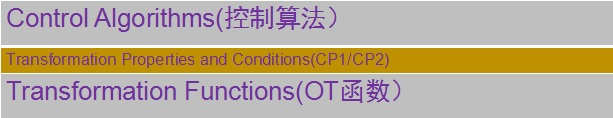
\includegraphics{figures/OT structure.jpg}
\caption{OT系统结构}
\end{figure}

控制算法负责决定哪些操作以何种顺序进行转换,而具体的OT函数则实施具体的两个操作之间的变化。
OT函数的数量由OT系统的模型所支持的数据和操作类型所决定。
这两者由一系列转换条件和属性结合在一起,所以整个OT系统的正确性就是由控制算法和OT函数的正确性以及协议的正确性所共同决定的。

由于这种分层结构,我们可以单独考虑OT函数的设计,而不必关心控制算法。
\cite{nichols1995high-latency}
\cite{sun2014exhaustive}
\section{应用背景:Redis 系统}
\subsection{Redis简介}
Redis是一个开源的、可基于内存也可持久化的数据结构存储系统,可以用作数据库、缓存和消息中间件,并且提供多种语言的API。Redis支持多种类型的数据结构,如字符串(string),散列(hash),列表(即本文中所关心的lists),集合(set),有序集合(sorted set)等
\subsection{Redis特点}
与其他key-value缓存产品相比,Redis具有以下的几个特点:
\begin{itemize}
\item Redis支持数据的持久化,可以在磁盘中保存内存里的数据
\item 除了简单的key-value型数据,Redis还提供多种数据结构的存储(包括List)
\item Redis支持主从模式的数据备份
\item 可以对Redis中的各种数据结构执行原子操作
\end{itemize}
\section{本文研究工作: 面向 Redis List的OT函数的设计与验证}
	\par 本次毕业设计的目标是实现Redis List所支持的14种非阻塞操作的OT(Operational Transformation)函数,并且对实现函数的正确性进行验证。阿里云和RedisLab的团队目前都在对Redis List的操作进行开发,Redis List操作的OT函数实现具有应用前景和商业前途。

	\par 在OT函数的设计方面,本文使用数学公式表示出所有OT函数的基本形式,并且绘制图片和表格进行相应说明。

	\par 在OT函数的验证方面,使用TLA +完成了对所设计OT函数的验证,证明其满足CP1正确性,并且对验证代码的复杂度进行了相应分析。
\section{论文组织}
	\par 本文后续内容组织如下:
	\par 第2章介绍本文的相关工作,包括系统模型和已有的相关OT函数的设计。
	\par 第3章介绍了Redis列表相关的基本命令,并对其进行了分类,然后进行了对应OT函数的设计。
	\par 第4章介绍了TLA+,并使用TLA+完成了对上述设计好的OT函数的验证,对实验结果进行了分析
	\par 第5章是本论文的结论和以后工作的相关展望。